\section{FEATURE ENGINEERING} 
\label{sec:feat-eng}

This section will describe the steps taken to pre-process the data and extract relevant features for our models. That includes which techniques that were chosen, how they work and why they were chosen. To conclude, a brief explanation of alternative techniques will be provided.

\subsection{SVM}

Before feeding the data into the Scikit-learn SVM algorithm, the data was flattened, changed into oriented gradient cells through HOG (Histogram of Oriented Gradient) and normalized (0-255 to 0-1 float). The HOG feature descriptor is used to differentiate between features through encoding interesting information into a numerical fingerprint made up of histogram gradients of some sort \cite{sklearn_api}. There are a lot of different feature descriptors, for instance, a SIFT descriptor, which computes oriented first order gradients, and the HOG descriptor, which on the other hand only computes a simple histogram of oriented gradients as the name implies. We chose to apply the latter, as a former is unnecessarily complex for our images and is better at describing the importance of a point. 

The before and after transforming the images to a HOG representation is shown in Figure \ref{fig:noHOG} and \ref{fig:HOG}. This feature extraction step proved to be a huge improvement for the accuracy of the model. Without transforming the images to HOG, it was 19,34\%. When transformed with the "default" HOG parameters (4 orientations, 2x2 cells and 1x1 block), it reached 72,39\%, and after tweaking the parameters (8 orientations, 4x4 cells and 1x1 block) it achieved  84,23\%. 

\begin{figure}[H] 
  \centering
  \begin{minipage}[b]{0.22\textwidth}
    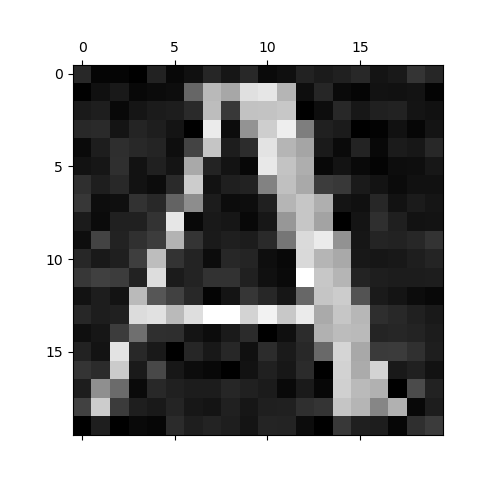
\includegraphics[width=\textwidth]{pictures/A_normalpng.png}
    \caption{Image before HOG.}
    \label{fig:noHOG}
  \end{minipage}
  \hfill
  \begin{minipage}[b]{0.22\textwidth}
    \includegraphics[width=\textwidth]{pictures/A_HOG.png}
    \caption{Image after HOG.}
    \label{fig:HOG}
  \end{minipage}
\end{figure}




\subsection{CNN}

Pre-processing for convolutional networks is executed in layers. Prior to the classification process, the data is reshaped with several techniques including \textit{convolutional, pooling} and \textit{dropout} layers.

% Convolutional layers
A convolutional layer systematically applies learned filters to the input images in order to create feature maps that summarize the presence of those features in the input \cite{Brownlee2019}. The approach is proven to be very effective, and stacking them in deep models allows the layers to learn abstract features like shapes and objects. This is very intuitive for our data, as recognizing line segments and curves are directly applicable for characters. However, the convolutional layers record the position of the features in the input with high precision. This means that even small distortions of the feature in an input image will result in a totally different feature map. Such changes are prone to happen when the input image is noised, shifted or rotated.

% Max pooling
To counteract the limitations of the convolutional layers, a subsequent Maximum pooling layer is added. Pooling helps to make the representation become approximately invariant to small translations of the input  \cite{Brownlee2019}. The layer will summarize the most activated presence of a feature to down-sample the feature map, like in Figure \ref{fig:maxP}. This way, the small movements detected by the convolutional layers will result in a pooled feature map with the feature located in the same place.

\begin{figure}[H]
    \centering
    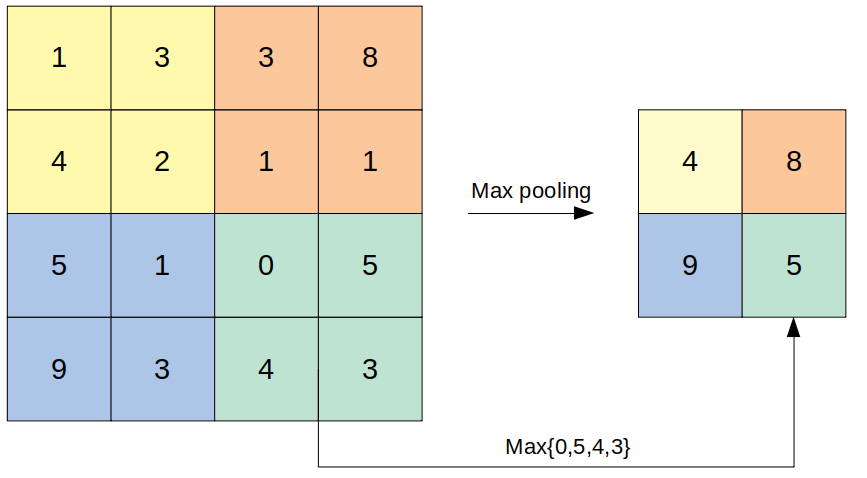
\includegraphics[width=0.45\textwidth]{pictures/maxPooling.png}
    \caption{Max Pooling process.}
    \label{fig:maxP}
\end{figure}

% Dropout to prevent overfitting
For further processing, a dropout layer is included. The dropout technique randomly selects neurons that will be neglected for the duration of the current iteration. It is believed that the network this way will learn multiple independent internal representations \cite{Brownlee2016}. Practically, the layer will drop out randomly selected features. The effect of dropout layers is a reduced chance of \textit{overfitting} as the network becomes less sensitive to specific weights of neurons.



\subsection{ALTERNATIVE TECHNIQUES}

Examining the images of the letters, they seem to be greyscale images where the contour of the letters fits snuggly inside the image frame. Hence, cropping were not a necessary measure, as the letters fit perfectly inside the frame.

The noise layers that can be applied with Keras seems very interesting for this task. Adding noise to a model with a small training dataset can reduce the chance of overfitting. Chars74k-lite has 7112 images in total, yielding 273 images per character which is prior to splitting them in training and test sets. Augmenting the dataset with noised images could prove to make the model more accurate. We did try to supplement the existing dataset with augmented data using a data generator tool from Keras, however it seemed to directly transform the data and not simply append it to our dataset. After completing the full machine learning project did we find a way to extend our dataset with augmented images, which it is not used in our code.

However, a tool from Keras called Data Generators were instead applied, which has the same purpose:  adding flipped, rotated and rescaled images. 

For the SVM we tried to convert to greyscale and apply a blur to remove possible "salt and pepper" noise (misplaced black and white dots), but it only seemed to decrease the accuracy by a few tenths.

Another method that were considered for the SVM was a Principal Component Analysis (PCA). PCA reduces the number of dimensions by projecting them onto a lower-dimensional sub-space \cite{scikit-learn}. For instance it would be possible to produce some kind of projection of the a-z letters onto a 3d plane, by finding the three variables that contains most of the information about the image. It would be cool to maybe try to plot them on a 3d graph, but we deemed it unnecessary.

